%!TEX program = xelatex
\documentclass[times,namecite]{goose-article}

\title{%
  GooseMaterial/AmorphousSolid/LinearStrain/ElastoPlastic
}

\author{T.W.J.~de~Geus}

\contact{%
  $^*$Contact: %
  \href{mailto:tom@geus.me}{tom@geus.me} %
  \hspace{1mm}--\hspace{1mm} %
  \href{http://www.geus.me}{www.geus.me}%
  \hspace{1mm}--\hspace{1mm} %
  \href{https://github.com/tdegeus/GooseMaterial}{https://github.com/tdegeus/GooseMaterial}%
}

\hypersetup{pdfauthor={T.W.J. de Geus}}

\header{%
  \href{https://github.com/tdegeus/GooseMaterial}{GooseMaterial/AmorphousSolid/LinearStrain/ElastoPlastic} -- \href{http://www.geus.me}{T.W.J.\ de Geus}%
}

\newcommand\leftstar[1]{\hspace*{-.3em}~^\star\!#1}

\begin{document}

\maketitle

\begin{abstract}
A microscopic continuum model of plasticity in amorphous solids is proposed. This model uses a strain energy with multiple minima to capture the effect of plasticity. This model is taken from the work of \citet{Jagla2017}.
\end{abstract}

\keywords{elasto-plasticity; linear elasticity}

\setcounter{tocdepth}{3}
\tableofcontents

\vfill\newpage
\section{General model}

\subsection{Constitutive model}

The model is constructed such that it behaves linear elastically in the volumetric stress response. The same holds for the deviatoric stress response, whereby plasticity is modeled such that the material starts flowing once a critical strain is reached. After a period of flow, the deviatoric stress response is again linear elastic. A detail to mention upfront, is that the elastic moduli and the equivalent stress and strain are defined such that the model is equivalent regardless of the number of dimensions, $d$, and it has the least amount of prefactors in the stress--strain response. To retrieve the common definitions in linear elasticity for $d = 3$, one simply has to scale these parameters (see Section~\ref{sec:nomenclature} for the nomenclature, including the parameter transformation).

The model is based on a strain energy $W$ is considered which is composed of two parts, a volumetric (or hydrostatic) part $U$ related to the hydrostatic strain $\varepsilon_\mathrm{m}$, and a shear (or deviatoric) part $V$ related to the equivalent strain $\varepsilon_\mathrm{eq}$, i.e.\
\begin{equation}
  W ( \bm{\varepsilon} ) = U ( \varepsilon_\mathrm{m} ) + V ( \varepsilon_\mathrm{eq} )
\end{equation}
The stress response $\bm{\sigma}$ is the derivative of this energy with respect to the strain tensor $\bm{\varepsilon}$. Before specializing $U$ and $V$ we can already say that
\begin{equation}\label{eq:dU-dV:elas}
  \bm{\sigma}
  =
  \frac{\partial W}{\partial \bm{\varepsilon}}
  =
  \frac{\partial U}{\partial \varepsilon_\mathrm{m}} \;
  \frac{\partial \varepsilon_\mathrm{m}}{\partial \bm{\varepsilon}}
  +
  \frac{\partial V}{\partial \varepsilon_\mathrm{eq}} \;
  \frac{\partial \varepsilon_\mathrm{eq}}{\partial \bm{\varepsilon}}
  =
  \frac{\partial U}{\partial \varepsilon_\mathrm{m}} \;
  \frac{1}{d} \bm{I}
  +
  \frac{\partial V}{\partial \varepsilon_\mathrm{eq}} \;
  \frac{\bm{\varepsilon}_d}{2 \, \varepsilon_\mathrm{eq}}
\end{equation}
From which we can identity the hydrostatic stress and the deviator stress tensor:
\begin{equation}\label{stress:generic}
  \sigma_\mathrm{m} = \frac{1}{d} \frac{\partial U}{\partial \varepsilon_\mathrm{m}}
  \;, \qquad
  \bm{\sigma}_\mathrm{d}
  =
  \frac{\partial V}{\partial \varepsilon_\mathrm{eq}} \;
  \frac{\bm{\varepsilon}_d}{2 \, \varepsilon_\mathrm{eq}}
\end{equation}

\subsubsection{Linear elasticity}

We start simple by considering linear elasticity. In this case the volumetric strain energy $U$ and the shear strain energy $V$ read
\begin{equation}\label{eq:W:elas}
  U ( \varepsilon_\mathrm{m}  ) = \frac{d}{2} \, K \, \varepsilon_\mathrm{m}^2
  \;, \qquad
  V ( \varepsilon_\mathrm{eq} ) = G \, \varepsilon_\mathrm{eq}^2
\end{equation}
The two potentials are plotted in Fig.~\ref{fig:U-V:elas} (in which only $\varepsilon_\mathrm{eq} \geq 0$ is shown, as it is by definition non-negative). It is trivial to obtain that
\begin{equation}
  \frac{\partial U}{\partial \varepsilon_\mathrm{m}}
  =
  d \, K \, \varepsilon_\mathrm{m}
  \;, \qquad
  \frac{\partial V}{\partial \varepsilon_\mathrm{eq}}
  =
  2 \, G \, \varepsilon_\mathrm{eq}
\end{equation}
(plotted in Fig.~\ref{fig:dU-dV:elas}). From which we obtain the following expression for the stress
\begin{equation}\label{eq:sig-elas}
  \bm{\sigma} ( \bm{\varepsilon} )
  =
  K \, \varepsilon_\mathrm{m} \, \bm{I}
  +
  G \, \bm{\varepsilon}_\mathrm{d}
\end{equation}

\begin{figure}[htp]
  \centering
  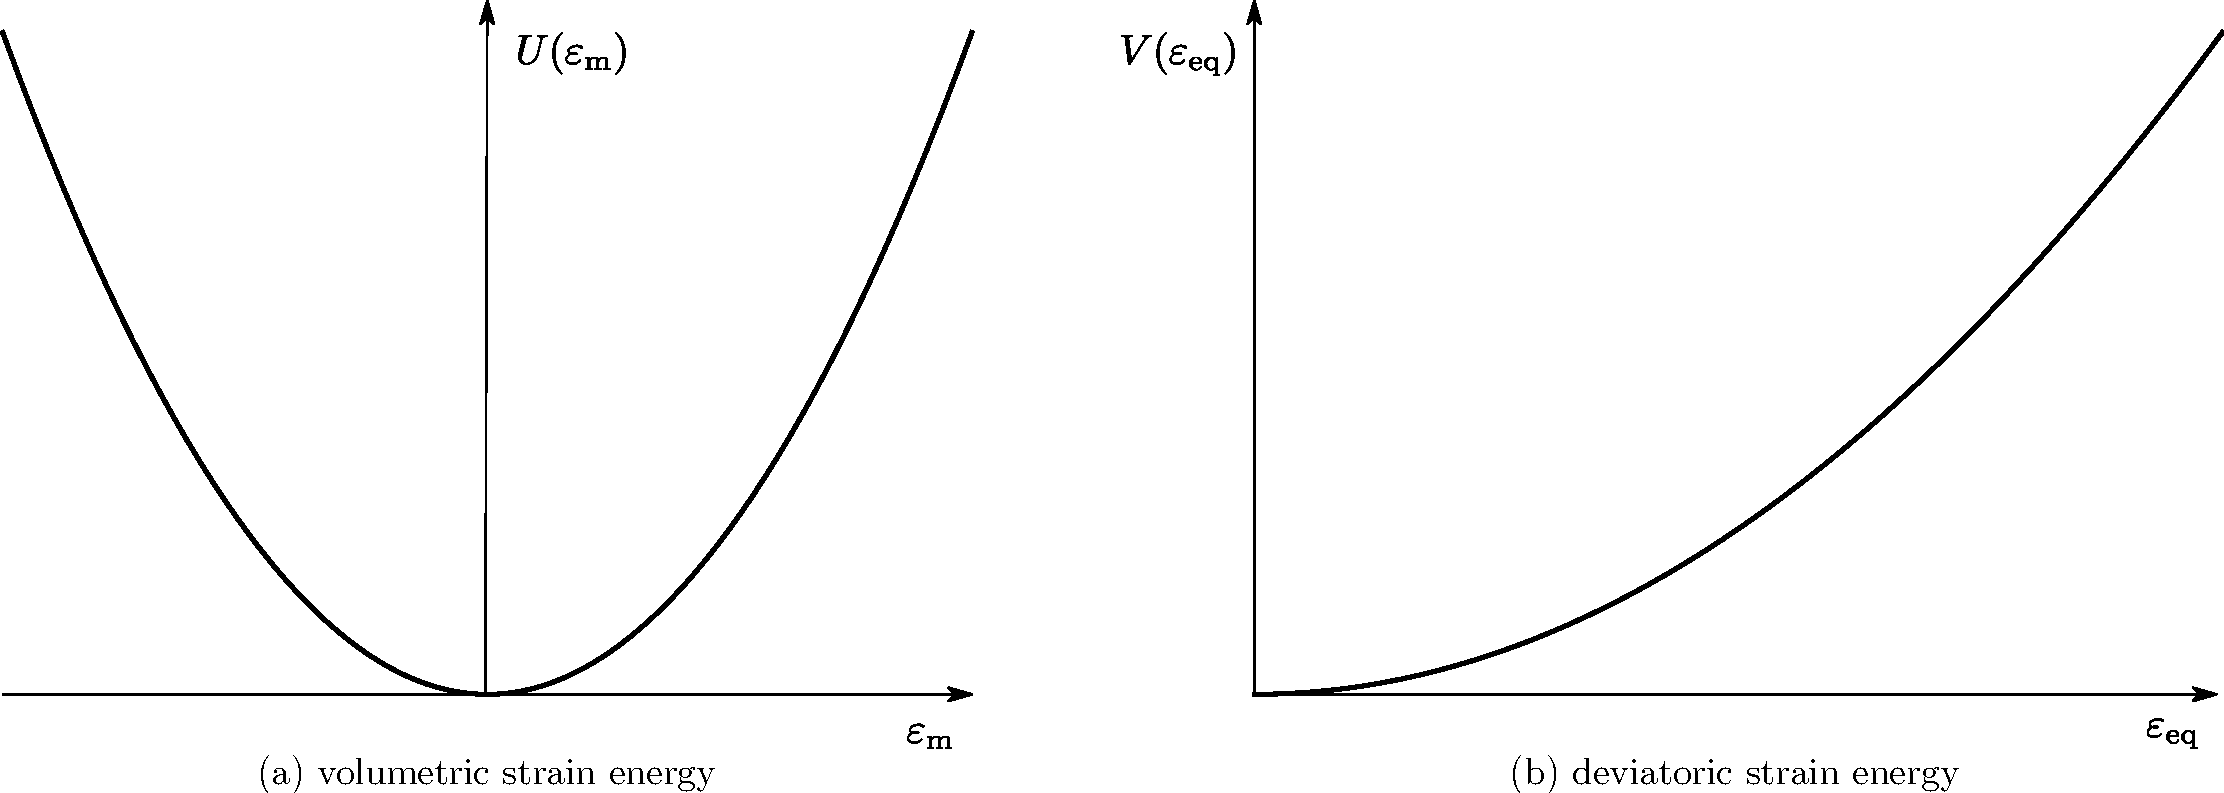
\includegraphics[width=1.\textwidth]{figures/potential_U-V_elas}
  \caption{Strain energy $W ( \bm{\varepsilon} ) = U ( \varepsilon_\mathrm{m} ) + V ( \varepsilon_\mathrm{eq} )$ for linear elasticity.}
  \label{fig:U-V:elas}
\end{figure}

\begin{figure}[htp]
  \centering
  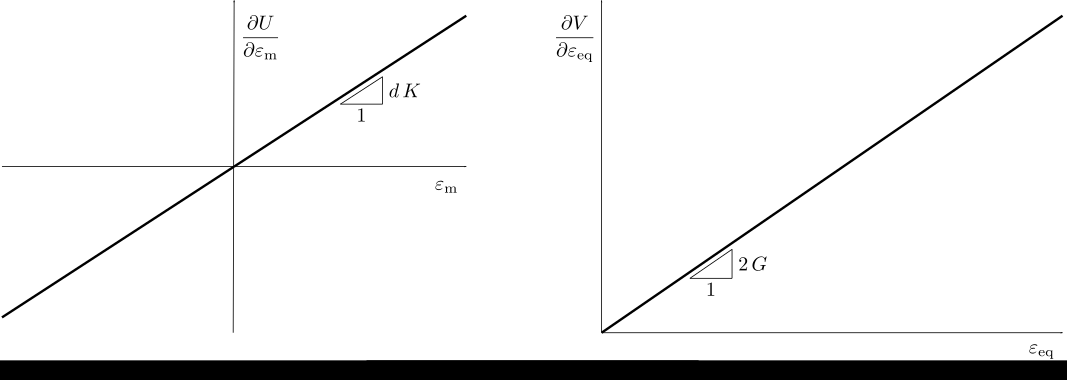
\includegraphics[width=1.\textwidth]{figures/potential_dU-dV_elas}
  \caption{Derivative of the hydrostatic strain energy $U$ and the deviatoric strain energy $V$ w.r.t.\ respectively the hydrostatic strain $\varepsilon_\mathrm{m}$ and the equivalent strain $\varepsilon_\mathrm{eq}$.}
  \label{fig:dU-dV:elas}
\end{figure}

\subsubsection{Plastic potential}

The model is now extended to account for plasticity. The model is defined such that the material responds volumetrically purely elastic, while in shear the model is governed by multiple minima. These minima have the effect that when the material reaches a certain yield stress it jumps to the next minimum. Around this minimum the elasticity is always the same. When loading is continued the the material again jumps to a new minimum when the next yield stress is reached. The magnitude of the jumps and of the yield stress are thereby related.

\paragraph{Parabolic potential with multiple minima}

As described, the volumetric behavior is simply elastic; given by Eq.~(\ref{eq:W:elas}a) and plotted in Fig.~\ref{fig:U-V:elas}(a). To attain the desired behavior in shear we divide the equivalent strain space in a finite number of yield strains $\varepsilon_\mathrm{y}^{(0)}, \varepsilon_\mathrm{y}^{(1)}, \varepsilon_\mathrm{y}^{(2)}, ...$ and define a parabolic potential between each pair ($[ \varepsilon_\mathrm{y}^{(0)}, \varepsilon_\mathrm{y}^{(1)} )$, $[ \varepsilon_\mathrm{y}^{(1)}, \varepsilon_\mathrm{y}^{(2)} )$, ...). The shear strain energy is then composed of a manifold of quadratic contributions
\begin{equation}\label{eq:V-plas}
  V \big(
    \varepsilon_\mathrm{y}^{(i)} \leq \varepsilon_\mathrm{eq} < \varepsilon_\mathrm{y}^{(i+1)}
  \big)
  =
  V^{(i)}
  =
  G \, \bigg[\,
    \Big[\, \varepsilon_\mathrm{eq} - \varepsilon_\mathrm{min}^{(i)} \,\Big]^2
    -
    \Big[\, \Delta \varepsilon_\mathrm{y}^{(i)} \,\Big]^2
  \,\bigg]
\end{equation}
where the mean of $\varepsilon_\mathrm{y}^{(i)}$ and $\varepsilon_\mathrm{y}^{(i+1)}$ is
\begin{equation}
  \varepsilon_\mathrm{min}^{(i)}
  =
  \frac{1}{2} \Big[\, \varepsilon_\mathrm{y}^{(i+1)} + \varepsilon_\mathrm{y}^{(i)} \,\Big]
\end{equation}
which is also the equivalent strain at which the shear strain energy reaches its minimum. From this minimum, the distance to $\varepsilon_\mathrm{y}^{(i)}$ and $\varepsilon_\mathrm{y}^{(i+1)}$ is
\begin{equation}
  \Delta \varepsilon_\mathrm{y}^{(i)}
  =
  \frac{1}{2} \Big[\, \varepsilon_\mathrm{y}^{(i+1)} - \varepsilon_\mathrm{y}^{(i)} \,\Big]
\end{equation}
The resulting shear strain energy is plotted in Fig.~\ref{fig:V:plas}(a).

The stress response is obtained from
\begin{equation}\label{eq:dV-plas}
  \frac{\partial V^{(i)}}{\partial \varepsilon_\mathrm{eq}}
  =
  2 \, G \, \Big[\, \varepsilon_\mathrm{eq} - \varepsilon_\mathrm{min}^{(i)} \,\Big]
\end{equation}
(see Fig.~\ref{fig:dV:plas}(a)). From which it can observed that in elasticity the behavior is identical to above (cf.~(\ref{eq:dU-dV:elas}b)). For the case that $\varepsilon_\mathrm{y}^{(0)} = - \varepsilon_\mathrm{y}^{(1)}$ the responses are even identical until initial yield stress is reached. For completeness, the stress reads
\begin{equation}
  \bm{\sigma} ( \bm{\varepsilon} )
  =
  K \, \varepsilon_\mathrm{m} \, \bm{I}
  +
  G \, \Big[\, 1 - \varepsilon_\mathrm{min}^{(i)} / \varepsilon_\mathrm{eq} \,\Big] \;
  \bm{\varepsilon}_\mathrm{d}
  \qquad
  \mathrm{for}
  \qquad
  \varepsilon_\mathrm{y}^{(i)} \leq \varepsilon_\mathrm{eq} < \varepsilon_\mathrm{y}^{(i+1)}
\end{equation}
whereby one has to assume that when $\varepsilon_\mathrm{eq} = 0$ also $\bm{\sigma}_\mathrm{d} = \bm{0}$ in order to avoid zero-devision.

From Fig.~\ref{fig:dV:plas}(a) we can observe that this model is not very realistic, as it exhibits stress jumps between different parabola in the potential, because of the discontinuity in the second derivative of the elastic potential. This is remedied in the final model, presented below.

\paragraph{Smooth parabolic potential with multiple minima}

The final model consists of a smoothened equivalent of Eq.~\eqref{eq:V-plas} is defined:
\begin{equation}\label{eq:V-plas-smooth}
  V \big(
    \varepsilon_\mathrm{y}^{(i)} \leq \varepsilon_\mathrm{eq} < \varepsilon_\mathrm{y}^{(i+1)}
  \big)
  =
  V^{(i)}
  =
  - 2 \, G \,
  \left[ \frac{\Delta \varepsilon_\mathrm{y}^{(i)}}{\pi} \right]^2
  \left[
    1
    +
    \cos \left(
      \frac{ \pi }{ \Delta \varepsilon_\mathrm{y}^{(i)} }
      \Big[\, \varepsilon_\mathrm{eq} - \varepsilon_\mathrm{min}^{(i)} \,\Big]
    \right)
  \right]
\end{equation}
which is plotted in Fig.~\ref{fig:V:plas}(b). In this case the stress is obtained from
\begin{equation}\label{eq:dV-plas-smooth}
  \frac{\partial V^{(i)}}{\partial \varepsilon_\mathrm{eq}}
  =
  2 \, G \,
  \left[ \frac{\Delta \varepsilon_\mathrm{y}^{(i)}}{\pi} \right]
  \sin \left(
    \frac{ \pi }{ \Delta \varepsilon_\mathrm{y}^{(i)} }
    \Big[\, \varepsilon_\mathrm{eq} - \varepsilon_\mathrm{min}^{(i)} \,\Big]
  \right)
\end{equation}
(see Fig.~\ref{fig:dV:plas}(b)). Which is to the first order equal to linear elasticity around its minimum $\varepsilon_\mathrm{min}^{(i)}$. Indeed, the first order Taylor series of Eq.~\eqref{eq:dV-plas-smooth} around $\varepsilon_\mathrm{eq} - \varepsilon_\mathrm{min}^{(i)} = 0$,
\begin{equation}
  \frac{\partial V^{(i)}}{\partial \varepsilon_\mathrm{eq}}
  \approx
  2 \, G \, \Big[\, \varepsilon_\mathrm{eq} - \varepsilon_\mathrm{min}^{(i)} \,\Big]
\end{equation}
is identical to Eq.~\eqref{eq:dV-plas}.

For completeness, also in case the expression for the entire stress tensor
\begin{equation}
  \bm{\sigma} ( \bm{\varepsilon} )
  =
  K \, \varepsilon_\mathrm{m} \, \bm{I}
  +
  G \,
  \left[ \frac{\Delta \varepsilon_\mathrm{y}^{(i)}}{\pi} \right]
  \sin \left(
    \frac{ \pi }{ \Delta \varepsilon_\mathrm{y}^{(i)} }
    \Big[\, \varepsilon_\mathrm{eq} - \varepsilon_\mathrm{min}^{(i)} \,\Big]
  \right)
  \frac{\bm{\varepsilon}_\mathrm{d}}{\varepsilon_\mathrm{eq}}
  \qquad
  \mathrm{for}
  \qquad
  \varepsilon_\mathrm{y}^{(i)} \leq \varepsilon_\mathrm{eq} < \varepsilon_\mathrm{y}^{(i+1)}
\end{equation}
whereby, again, one has to assume that when $\varepsilon_\mathrm{eq} = 0$ also $\bm{\sigma}_\mathrm{d} = \bm{0}$ in order to avoid zero-devision.

\begin{figure}[htp]
  \centering
  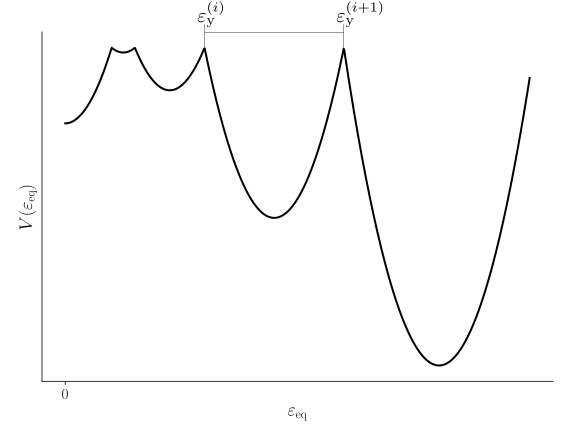
\includegraphics[width=1.\textwidth]{figures/potential_V-plas}
  \caption{The multi-minima shear strain energy, $V ( \varepsilon_\mathrm{eq} )$, that models the effect of plasticity. The multi-parabolic shear strain energy is shown in (a), while its smoothened equivalent is shown in (b).}
  \label{fig:V:plas}
\end{figure}

\begin{figure}[htp]
  \centering
  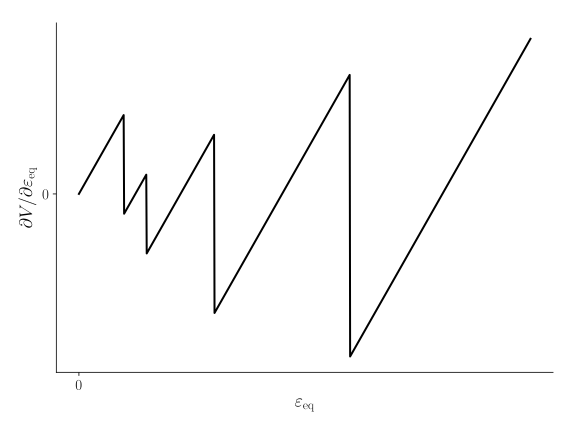
\includegraphics[width=1.\textwidth]{figures/potential_dV-plas}
  \caption{Derivative of the shear strain energy $V$.}
  \label{fig:dV:plas}
\end{figure}

\subsection{Nomenclature}
\label{sec:nomenclature}

\subsubsection{Tensor products}
\label{sec:nomenclature:tensor}

\begin{itemize}
%
\item Dyadic tensor product
\begin{align}
  \mathbb{C} &= \bm{A} \otimes \bm{B} \\
  C_{ijkl}   &= A_{ij} \,      B_{kl}
\end{align}
%
\item Double tensor contraction
\begin{align}
  C &= \bm{A} : \bm{B} \\
    &= A_{ij} \, B_{ji}
\end{align}
%
\item Deviatoric projection tensor (in $d$ dimensions)
\begin{equation}
  \mathbb{I}_\mathrm{d}
  = \mathbb{I}_\mathrm{s} - \tfrac{1}{d} \bm{I} \otimes \bm{I}
\end{equation}
%
\end{itemize}

\subsubsection{Strain measures}
\label{sec:nomenclature::strain}

\begin{itemize}
%
\item Mean strain (in $d$ dimensions)
\begin{equation}
  \varepsilon_\mathrm{m}
  = \tfrac{1}{d} \, \mathrm{tr} ( \bm{\varepsilon} )
  = \tfrac{1}{d} \, \bm{\varepsilon} : \bm{I}
\end{equation}
%
\item Strain deviator
\begin{equation}
  \bm{\varepsilon}_\mathrm{d}
  = \bm{\varepsilon} - \varepsilon_\mathrm{m} \, \bm{I}
  = \mathbb{I}_\mathrm{d} : \bm{\varepsilon}
\end{equation}
%
\item Equivalent strain
\begin{equation}
  \varepsilon_\mathrm{eq}
  = \; \sqrt{
    \tfrac{1}{2} \, \bm{\varepsilon}_\mathrm{d} : \bm{\varepsilon}_\mathrm{d}
  }
\end{equation}
%
\end{itemize}

\subsubsection{Stress measures}
\label{sec:nomenclature::stress}

\begin{itemize}
%
\item Mean stress (in $d$ dimensions)
%
\begin{equation}
\sigma_\mathrm{m}
= \tfrac{1}{d} \, \mathrm{tr} ( \bm{\sigma} )
= \tfrac{1}{d} \, \bm{\sigma} : \bm{I}
\end{equation}
%
\item Stress deviator
%
\begin{equation}
  \bm{\sigma}_\mathrm{d}
  = \bm{\sigma} - \sigma_\mathrm{m} \, \bm{I}
  = \mathbb{I}_\mathrm{d} : \bm{\sigma}
\end{equation}
%
\item Von Mises equivalent stress
\begin{equation}
\sigma_\mathrm{eq} = \sqrt{ \tfrac{1}{2} \, \bm{\sigma}_\mathrm{d} : \bm{\sigma}_\mathrm{d} }
\end{equation}
%
\end{itemize}

\subsubsection{Derivatives}
\label{sec:nomenclature:derivatives}

\begin{itemize}
%
\item Strain deviator
\begin{equation}
  \frac{ \partial \bm{\varepsilon}_\mathrm{d} }{ \partial \bm{\varepsilon} }
  = \mathbb{I}_\mathrm{d}
\end{equation}
%
\item Mean equivalent strain (in $d$ dimensions)
\begin{equation}
  \frac{ \partial \varepsilon_\mathrm{m} }{ \partial \bm{\varepsilon} }
  =
  \tfrac{1}{d} \bm{I} : \mathbb{I}
  =
  \tfrac{1}{d} \bm{I}
\end{equation}
%
\item Von Mises equivalent strain
\begin{equation}
  \frac{ \partial \varepsilon_\mathrm{eq} }{ \partial \bm{\varepsilon} }
  =
  \frac{1}{2 \, \varepsilon_\mathrm{eq}} \frac{1}{2}
  \big[\, \mathbb{I}_\mathrm{d} : \bm{\varepsilon}_\mathrm{d} + \bm{\varepsilon}_\mathrm{d} : \mathbb{I}_\mathrm{d} \,\big]
  =
  \frac{\bm{\varepsilon}_\mathrm{d}}{2 \, \varepsilon_\mathrm{eq}}
\end{equation}
%
\end{itemize}

\subsubsection{Conversion to common parameters for linear elasticity}

Here the parameters are confronted to their common definitions (denoted here with a tilde) for linear elasticity in $d = 3$:

\begin{itemize}
  \item Hydrostatic strain
  \begin{equation}
    \tilde{\varepsilon}_\mathrm{m} = \varepsilon_\mathrm{m}
  \end{equation}
  \item Equivalent strain
  \begin{equation}
    \tilde{\varepsilon}_\mathrm{eq}
    = \sqrt{\tfrac{2}{3} \bm{\varepsilon}_\mathrm{d} : \bm{\varepsilon}_\mathrm{d} }
    = \sqrt{\tfrac{4}{3}} \; \varepsilon_\mathrm{eq}
  \end{equation}
  \item Hydrostatic stress
  \begin{equation}
    \tilde{\sigma}_\mathrm{m} = \sigma_\mathrm{m}
  \end{equation}
  \item Equivalent stress
  \begin{equation}
    \tilde{\sigma}_\mathrm{eq}
    = \sqrt{\tfrac{3}{2} \bm{\sigma}_\mathrm{d} : \bm{\sigma}_\mathrm{d} }
    = \sqrt{3} \; \sigma_\mathrm{eq}
  \end{equation}
  \item Bulk modulus
  \begin{equation}
    \tilde{K} = 3 \, K
  \end{equation}
  \item Shear modulus
  \begin{equation}
    \tilde{G} = 2 \, G
  \end{equation}
\end{itemize}
This results in a stress response
\begin{equation}
  \bm{\sigma} ( \bm{\varepsilon} )
  =
  3 K \, \varepsilon_\mathrm{m} \, \bm{I}
  +
  2 G \, \bm{\varepsilon}_\mathrm{d}
\end{equation}
Note the the equivalent stress and strain are defined such that they are work conjugate (i.e. $\sigma_\mathrm{eq} \, \varepsilon_\mathrm{eq} = \bm{\sigma} : \bm{\varepsilon}$) for uniaxial extension of an incompressible material.

\bibliography{library}

\end{document}
